\documentclass[tikz,border=10pt]{standalone}
\usepackage{amsmath,amssymb}
\usepackage{pgfplots}
\pgfplotsset{compat=1.18}
\usetikzlibrary{arrows.meta,positioning,calc,shapes}

\definecolor{politoNavy}{RGB}{0, 43, 91}
\definecolor{deepdiveTeal}{RGB}{0, 128, 128}
\definecolor{examred}{RGB}{180, 40, 40}
\definecolor{intuitiongreen}{RGB}{40, 130, 80}

\begin{document}
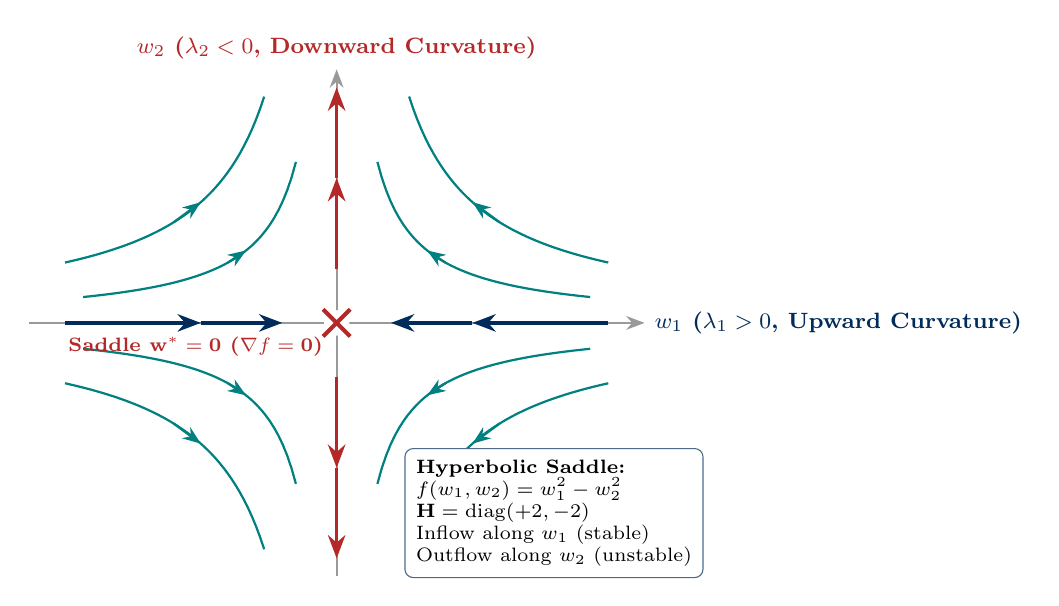
\begin{tikzpicture}[>=Stealth, scale=1.15]
  % Axes
  \draw[->, thick, gray!80] (-3.4, 0) -- (3.4, 0) node[right, font=\footnotesize\bfseries, text=politoNavy] {$w_1$ ($\lambda_1 > 0$, Upward Curvature)};
  \draw[->, thick, gray!80] (0, -2.8) -- (0, 2.8) node[above, font=\footnotesize\bfseries, text=examred] {$w_2$ ($\lambda_2 < 0$, Downward Curvature)};

  % Inflow arrows along w1 axis (Stable manifold)
  \draw[->, very thick, politoNavy] (3.0, 0) -- (1.5, 0);
  \draw[->, very thick, politoNavy] (1.5, 0) -- (0.6, 0);
  \draw[->, very thick, politoNavy] (-3.0, 0) -- (-1.5, 0);
  \draw[->, very thick, politoNavy] (-1.5, 0) -- (-0.6, 0);

  % Outflow arrows along w2 axis (Unstable manifold)
  \draw[->, very thick, examred] (0, 0.6) -- (0, 1.6);
  \draw[->, very thick, examred] (0, 1.6) -- (0, 2.6);
  \draw[->, very thick, examred] (0, -0.6) -- (0, -1.6);
  \draw[->, very thick, examred] (0, -1.6) -- (0, -2.6);

  % Hyperbolic streamlines in quadrants
  % Quadrant 1
  \draw[thick, deepdiveTeal, domain=0.45:2.8, samples=50] plot (\x, {0.8/\x});
  \draw[->, thick, deepdiveTeal] (1.2, {0.8/1.2}) -- (1.0, {0.8/1.0});

  \draw[thick, deepdiveTeal, domain=0.8:3.0, samples=50] plot (\x, {2.0/\x});
  \draw[->, thick, deepdiveTeal] (1.8, {2.0/1.8}) -- (1.5, {2.0/1.5});

  % Quadrant 2
  \draw[thick, deepdiveTeal, domain=-2.8:-0.45, samples=50] plot (\x, {-0.8/\x});
  \draw[->, thick, deepdiveTeal] (-1.2, {-0.8/-1.2}) -- (-1.0, {-0.8/-1.0});

  \draw[thick, deepdiveTeal, domain=-3.0:-0.8, samples=50] plot (\x, {-2.0/\x});
  \draw[->, thick, deepdiveTeal] (-1.8, {-2.0/-1.8}) -- (-1.5, {-2.0/-1.5});

  % Quadrant 3
  \draw[thick, deepdiveTeal, domain=-2.8:-0.45, samples=50] plot (\x, {0.8/\x});
  \draw[->, thick, deepdiveTeal] (-1.2, {0.8/-1.2}) -- (-1.0, {0.8/-1.0});

  \draw[thick, deepdiveTeal, domain=-3.0:-0.8, samples=50] plot (\x, {2.0/\x});
  \draw[->, thick, deepdiveTeal] (-1.8, {2.0/-1.8}) -- (-1.5, {2.0/-1.5});

  % Quadrant 4
  \draw[thick, deepdiveTeal, domain=0.45:2.8, samples=50] plot (\x, {-0.8/\x});
  \draw[->, thick, deepdiveTeal] (1.2, {-0.8/1.2}) -- (1.0, {-0.8/1.0});

  \draw[thick, deepdiveTeal, domain=0.8:3.0, samples=50] plot (\x, {-2.0/\x});
  \draw[->, thick, deepdiveTeal] (1.8, {-2.0/1.8}) -- (1.5, {-2.0/1.5});

  % Critical saddle point at origin
  \fill[white] (0,0) circle (4pt);
  \draw[line width=1.5pt, examred] (-0.15, -0.15) -- (0.15, 0.15);
  \draw[line width=1.5pt, examred] (-0.15, 0.15) -- (0.15, -0.15);
  \node[below left=2pt, font=\scriptsize\bfseries, text=examred] at (0,0) {Saddle $\mathbf{w}^* = \mathbf{0}$ ($\nabla f = \mathbf{0}$)};

  % Annotation callout
  \node[draw=politoNavy!70, fill=white, rounded corners=3pt, font=\scriptsize, align=left, inner sep=4pt] at (2.4, -2.1) {
    \textbf{Hyperbolic Saddle:}\\
    $f(w_1, w_2) = w_1^2 - w_2^2$\\
    $\mathbf{H} = \mathrm{diag}(+2, -2)$\\
    Inflow along $w_1$ (stable)\\
    Outflow along $w_2$ (unstable)
  };
\end{tikzpicture}
\end{document}
